\documentclass[11pt, a4paper]{article}

\usepackage{amsmath}
\usepackage{amsfonts}
\usepackage{graphicx}
\usepackage[export]{adjustbox}
\usepackage{hyperref}
\usepackage{fullpage}
\usepackage{caption}
\usepackage{listings}
\usepackage[dvipsnames]{xcolor}
\usepackage{gensymb}
\hypersetup{
    bookmarks=true,         % show bookmarks bar?
    unicode=false,          % non-Latin characters in Acrobat’s bookmarks
    pdftoolbar=true,        % show Acrobat’s toolbar?
    pdfmenubar=true,        % show Acrobat’s menu?
    pdffitwindow=false,     % window fit to page when opened
    pdfstartview={FitH},    % fits the width of the page to the window
    pdftitle={My title},    % title
    pdfauthor={Author},     % author
    pdfsubject={Subject},   % subject of the document
    pdfcreator={Creator},   % creator of the document
    pdfproducer={Producer}, % producer of the document
    pdfkeywords={keyword1, key2, key3}, % list of keywords
    pdfnewwindow=true,      % links in new PDF window
    colorlinks=true,       % false: boxed links; true: colored links
    linkcolor=Blue,          % color of internal links (change box color with linkbordercolor)
    citecolor=green,        % color of links to bibliography
    filecolor=magenta,      % color of file links
    urlcolor=red           % color of external links
}

\title{MAAS - Project Report \\Commitment Issues}
\author{Sushant Vijay Chavan\\Ahmed Faisal Abdelrahman\\Abanoub Abdelmalak}
\date{\today}

\begin{document}
\maketitle
\newpage
\tableofcontents{}
\newpage

\section{Introduction}
This project was completed as a part of the project work for the Multi-Agent and Agent Systems course. In this project we implemented two stages (Packaging and Delivery) of the Flying Saucers Bakery project. In addition we implemented visualization of the delivery stage as a street network with moving trucks to show the delivery in action. 

\textbf{TODO}

\section{Packaging Stage}\label{PackagingStage}
\paragraph{}
This stage deals with completion of the post baking stages and then packaging the products into boxes so that they are ready for delivery. The stage receives the baked and cooled products from the cooling racks and preforms the final preparation of the products such as sprinkling and decorating according to the recipe for the product. Once the products are ready, they are packed into boxes based on the delivery date priority of the orders. Once all the boxes of a given product type in an order are ready, they are sent to the delivery stage for transportation.

\paragraph{}
Figure \ref{PackagingArchitecture} gives an overview of the architecture of the packaging stage. This stage consists of three agents and in addition communicates with the CoolingRacks agent to receive the cooled products. The GenericItemProcessor takes care of all the post-baking steps, where as the packaging agent boxes the products based on the order priority. The Loading bay keeps track of the produced quantity of the products and informs the delivery stage whenever all products of a type in an order are ready.

\begin{figure}[h!]
	\centering
	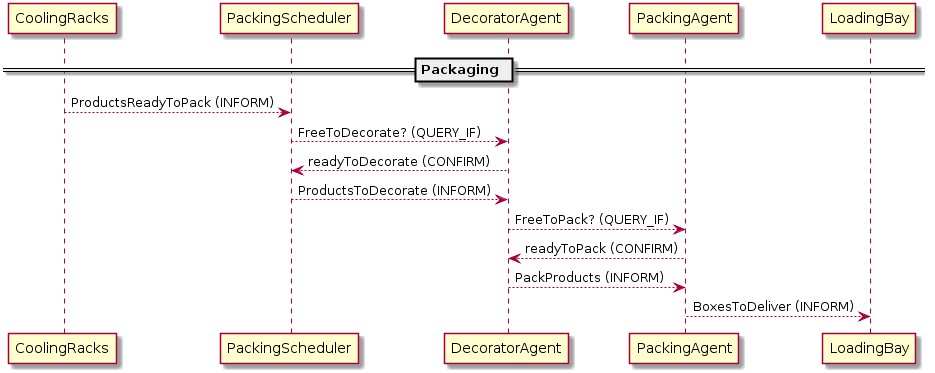
\includegraphics[width=\textwidth]{../Architecture/Architecture_Packaging.png}
	\caption{Packaging Stage Architecture}
	\label{PackagingArchitecture}
\end{figure}

\paragraph{}
The output of this stage is a set of boxes that consists of a fulfilled item from a customer order. For example, if a customer order consists of 10 breads and 15 donuts, assuming that the loading bay sees that the 15 donuts of this order are available, it sends these boxes to the delivery stage. Please note that not all products of this order are yet complete and that the loading bay will wait until all the breads of this order are available before sending out a new message to the delivery stage.

\hfill\break
\subsection{Agents}\label{PackagingAgents}
\begin{enumerate}
	\item \textit{Generic Item Processor} (Owner: Abanoub):\\
	This agent is responsible for receiving the items sent by the cooling racks, prepare them for packaging and send them to the packaging agent to be packed. Based on the scenario files used for the simulation and the bakery this agent belongs to, it creates a list with all the products. Using the scenario file, each product is acquired with the processes it needs to be ready for packaging and their duration. After preparing this list of the products with their features, the agent starts to receive products from the cooling racks and start executing the processes one by one for each of them until it is done. The products are sent to the packaging agent as soon as they are processed and all the time needed for each of the processes is finished.
	\item \textit{Packaging agent} (Owner: Sushant):
	\paragraph{}
	This agent is responsible for receiving the ready products and then packaging them into boxes. The packaged boxes are then sent to the loading bay so that they can be dispatched to the customer. This agent prioritizes the packaging of the received products based on the delivery time of the orders. 
	\paragraph{}
	For example, assume we have two orders requiring 10 and 20 breads respectively and that the delivery date of the first order is earlier than that of the second. Now if we receive 20 breads from the previous stage, the packaging agents first boxes the 10 breads for the first order and sends them to the LoadingBay. It then packages the remaining 10 breads as a part of the second order. It must be noted that the packaging agent sends out the boxes as soon as they are full. It expects the loading bay to store the boxes until all boxes of a product in an order are ready.
	\item \textit{Loading Bay} (Owner: Ahmed):
%	Description and message description
	\paragraph{}
	The loading bay agent acts as the interface between the packaging phase and the delivery phase. Aside from transferring boxes of packaged products along from the packaging agent to the order aggregator agent, it is responsible for sending boxes of products only when all of the products of a respective order have been fulfilled.
	\paragraph{}
	The agent receives two types of messages, one from the preceding packaging agent and another from the common order processing agent. The former sends a list of boxes of products that belong to an order, while the latter provides the list of products needed to fulfill every order, among the other order details. The agent receives boxes of products and retains them with their order IDS. Meanwhile, it maintains all orders' details and continuously checks if it has all the products needed for any order. Once an order's products are all present, it dispatches a message to the next agent containing a list of all the boxes of products needed for a particular order.
	
	Message Descriptions:
	
	(Incoming) Packaged Boxes Message:
	
	The LoadingBayAgent receives boxes of packaged products from a packaging agent in a message of the following format:
	
	\textbf{Performative}: INFORM
	
	\textbf{Sender}: AID of the packaging agent
	
	\textbf{Receiver}: AID of the LoadingBayAgent
	
	\textbf{Conversation ID}: "boxes-ready"
	
	Figure \ref{loadingbaymsg1example} shows an example of the contents of the message.
	\begin{figure}[h!]
		\centering
		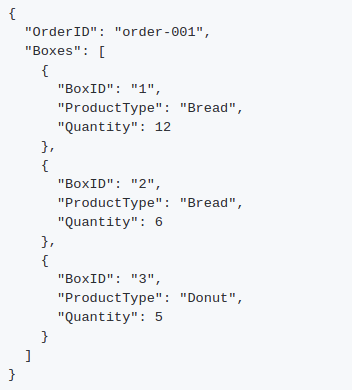
\includegraphics[width=0.4\textwidth]{../images/loadingbaymsg1example.png}
		\caption{Packaged Boxes Example Message}
		\label{loadingbaymsg1example}
	\end{figure}
	
	(Outgoing) Fulfilled Order Boxes Message:
	
	The LoadingBayAgent agent sends an order aggregator agent a message containing the details of boxes of products belonging to a particular order. It does so once it receives boxes that contain all of the products that fulfill that order. The message is of the following format:
	
	\textbf{Performative}: INFORM
	
	\textbf{Sender}: AID of the LoadingBayAgent
	
	\textbf{Receiver}: AID of an OrderAggregatorAgent
	
	The message is of the same format as the incoming message, and an example can be seen on Figure \ref{loadingbaymsg1example}.
	
\end{enumerate}

\newpage
\section{Delivery Stage}\label{DeliveryStage}
\paragraph{}
This stage handles the delivery of the packaged boxes from the bakery to the customers. The inputs to this stage are a set of boxes from the packaging stage as described in the section \ref{PackagingStage}. This stage waits until all the products of an order are ready for dispatch and then requests the trucks for transportation of these boxes. Once the orders have been delivered to the customer, the trucks post the status of the delivery to the mailbox, which then informs all agents that are interested in this information.

\paragraph{}
This stage consists of 5 agents as shown the architecture diagram in figure \ref{DeliveryArchitecture}. In addition this stage talks with two other agents: \textit{LoadingBayAgent} and the \textit{GraphVisualizationAgent}. The figure gives an overview of the communication happening between the agents in order to complete an order received from the LoadingBayAgent. The visualization of the delivery stage will be explained in detail in section \ref{GraphVisualizationAgent}. However it is helpful to know that the only agents that need to communicate with the GraphVisualizationAgent are the StreetNetworkAgent and the TruckAgents. 

\begin{figure}[h!]
	\centering
	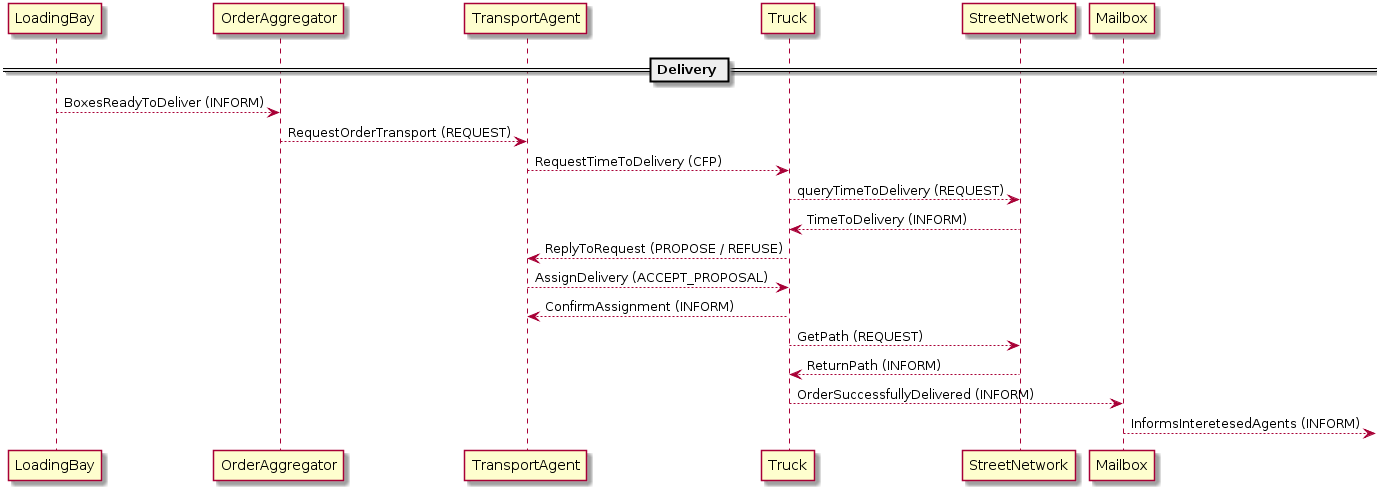
\includegraphics[width=\textwidth]{../Architecture/Architecture_Delivery.png}
	\caption{Delivery Stage Architecture}
	\label{DeliveryArchitecture}
\end{figure}

\paragraph{}
In order to find the best truck that can deliver the orders, the transport agent of the bakery requests for proposals from the trucks to deliver the order. Each Truck which is capable of delivery this order then queries the StreetNetwork to find the time needed by it to complete its current task and then return to the bakery to collect the products and then move towards the customer. These estimates are then sent back to the transport agent, which then chooses that truck that has the least time to delivery.  Section \ref{DeliveryAgents} provides a detailed description of all the agents that are a part of the delivery stage.

\subsection{Agents}\label{DeliveryAgents}
\begin{enumerate}
	\item \textit{OrderAggregator} (Owner: Abanoub):\\
	 Based on the idea that the loading bay will send the boxes of products that are complete, this agent is responsible for gathering all the needed information about the boxes sent by the loading bay and forward the complete orders to the transport agent after it makes sure that the order is fulfilled. The agent works as follows: it keeps track of all the orders that the order processor broadcast. Then it waits until the loading bay sends boxes to be delivered. The boxes with their order id are used to check the order fulfillment and then send the full order to the transport agent.
	\item \textit{TransportAgent} (Owner: Abanoub):\\
	This agent is responsible for receiving the boxes of fulfilled orders from the order aggregator, getting the location of the bakeries and the customers of this specific order, assigning the order to the trucks with the best delivery time and handing the orders to the trucks when they arrive at the bakeries. This is achieved as follows: It keeps updating a list of customers ids associated with their orders ids sent by the order processor. Then the cycle starts when it receives boxes from the order aggregator. It uses the details sent by the order aggregator to find the location of the customer and the bakery associated with this order. After that it communicates with all the trucks working under the the same transport company to call for proposals with the time each of them needs to deliver the order then chooses the truck with the best time and assigns the order to it. When the truck arrives at the bakery to pick the order it gives the order to it.\\
	Each transport agent and group of trucks are associated with one transport company.
	\item \textit{TruckAgent} (Owner: Sushant):\\
	This agent is responsible for collecting orders from a bakery and delivering them to the customers. Each truck is associated with a transport company and multiple transport companies could exist. It is responsible for querying the estimated delivery time for an order and proposing this to the transport agent. If the proposal is accepted, it is also responsible for moving towards the bakery to collect the orders and the move towards the customers to deliver them. Finally it also informs the status of the delivery (such as the time of delivery, number of boxes) to the mailbox. Due to its highly dynamic nature, this agent has an extensive communication with other agents, as can be seen from the figure \ref{DeliveryArchitecture}. It must be noted that with the current implementation, every truck can accept atmost one extra order in addition to the one it is currently handling. 
	
	Additionally this agent also communicates with the GraphVisualizationAgent in order to send its position and status updates for visualization. 
	\item \textit{StreetNetworkAgent} (Owner: Ahmed):
	\paragraph{}
	The street network agent is responsible for maintaining the world 'map' in a graphical representation, containing the locations of all places, connections between them, and the distances, as specified in each scenario. Additionally, it provides navigational and temporal information to truck agents. This includes the paths that they must traverse to get from one location to another, and the time it would take to do so.
	\paragraph{}
	With the help of a few helper classes, such as \textit{Graph}, \textit{Vertex}, and \textit{Edge}, the agent stores and updates (if necessary) the map as a directed graph. It makes use of an implementation of the Dijkstra algorithm that facilitates a graph search to find the shortest path between two nodes. This implementation is adapted from Lars Vogel's, which can be found \href{http://www.vogella.com/tutorials/JavaAlgorithmsDijkstra/article.html}{in this link}.
	\paragraph{}
	The agent communicates with truck agents and the graph visualization agent. The graph visualization agent constructs the visualization of the street network by obtaining the graph representation of the map from the street network agent.
	\item \textit{Mailbox} (Owner: Ahmed):
%	Description and message description
	\paragraph{}
	The mail box agent is the interface agent between the final delivery stage and the customers. It receives the details of delivered orders from truck agents, and confirms these deliveries to the concerned customer agents. It can be extended to relay this information to any agent who requires it.
	\paragraph{}
	The agent constructs a message whose types are defined in a class called \textit{DeliveryStatus}. The class contains all the relevant details of a confirmed delivery, such as the truck (and delivery company) that delivered it, the customer, the time, and the contents of the delivery.
	
	Message Descriptions:
	
	(Incoming) Truck Message:
	
	The TruckAgent informs the mailbox about a delivered order using the following message:
	
	\textbf{Performative}: INFORM
	
	\textbf{Sender}: AID of the TruckAgent that sends this message
	
	\textbf{Receiver}: AID of the MailboxAgent
	
	\textbf{PostTimeStamp}: Current system time
	
	\textbf{Conversation ID}: \textit{orderID}
	
	Figure \ref{mailboxmsgexample} shows an example of the contents of the message
	
	(Outgoing) Fulfilled Order Boxes Message:
	
	The mail box relays the delivery status message to the concerned customer and other agents who are interested in knowing the delivery status of the order using the following message:
	
	\textbf{Performative}: INFORM
	
	\textbf{Sender}: AID of the MailboxAgent
	
	\textbf{Receiver}: AID of the Concerned CutomerAgent. If more agents are interested in receiving this message, their AID's will also be added to the receiver list.
	
	\textbf{PostTimeStamp}: Current system time
	
	\textbf{Conversation ID}: \textit{orderID}
	
	The message is of the same format as the incoming message, and an example can be seen on Figure \ref{mailboxmsgexample}.
	
	TODO: ADD UPDATED MAILBOX MESSAGE
%	\begin{figure}[h!]
%		\centering
%		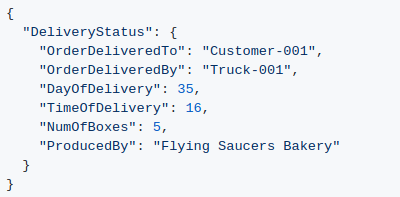
\includegraphics[width=0.4\textwidth]{../images/mailboxmsgexample.png}
%		\caption{Mailbox Example Message}
%		\label{mailboxmsgexample}
%	\end{figure}
\end{enumerate}

\newpage
\subsection{Graph Visualization Agent}\label{GraphVisualizationAgent}
Screenshot of the graph along with short description. Add reference to the codes source. 
\\Owners: All

\begin{figure}[h!]
	\centering
	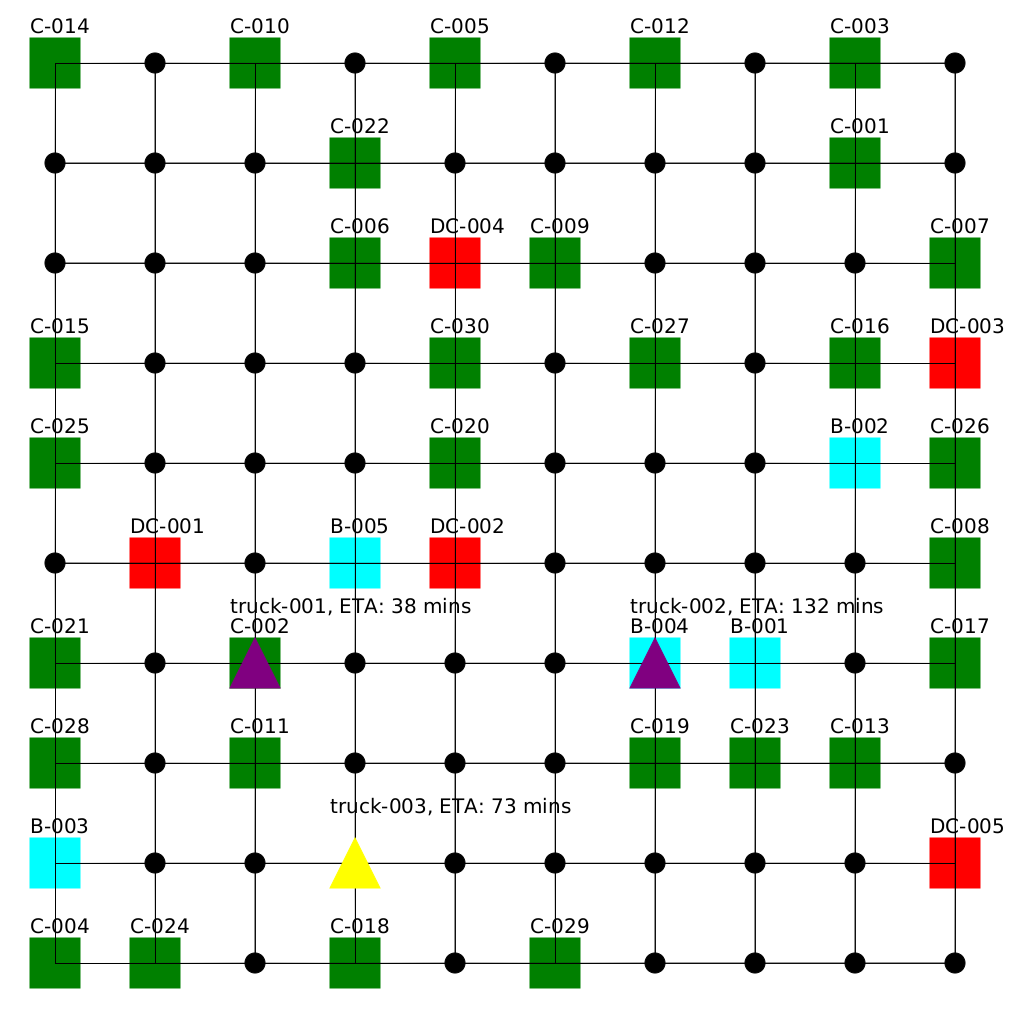
\includegraphics[width=\textwidth]{Visualization.png}
	\caption{Visualization Screenshot}
	\label{PackagingArchitecture}
\end{figure}

\newpage
\section{Entry Agent}
Owner: Sushant
\paragraph{}
In order to test the two developed stages independent of the other stages, we need an agent that can trigger the first agent of the cooling racks agent to start the simulation. The EntryAgents fulfills this requirement. Using this agent, it is possible to simulate that the products from of an order have been baked and are ready for cooling, which then starts the two following stages until the order has been delivered to the customer. It should be noted that the EntryAgent simply uses the order information available in the scenario files and does not generate any data on its own.

\paragraph{}
The Entry agent has two functionalities. First, it reads the order details from the currently active scenario directory and then generates dummy messages that inform the cooling rack that the products of an order are ready. These messages are then sent to the cooling rack at the delivery time mentioned in the scenario file. Therefore the first part of this agent acts as the trigger for the two stages. Since the order processor agent was also not available on the upstream repository, we added the order processor functionality as the second functionality of the entry agent. Whenever an order is sent to the cooling rack, a corresponding order information is also broadcasted to all agents. We used the same  message format as the actual order processor. This way we ensure that all our agents are compatible with the actual order processor, whenever it is available.

\section{Usage Instructions}

\subsection{Running the two stages}

\subsection{Running on distributed systems}

\section{Conclusion}

\end{document}\grid
